\documentclass[conference]{IEEEtran}
\IEEEoverridecommandlockouts
% The preceding line is only needed to identify funding in the first footnote. If that is unneeded, please comment it out.
\usepackage{cite}
\usepackage{amsmath,amssymb,amsfonts}
\usepackage{algorithmic}
\usepackage{graphicx}
\usepackage{textcomp}
\usepackage{xcolor}
\def\BibTeX{{\rm B\kern-.05em{\sc i\kern-.025em b}\kern-.08em
    T\kern-.1667em\lower.7ex\hbox{E}\kern-.125emX}}
\begin{document}

\title{A Survey of Security Issues in Federated Laearning}

\author{\IEEEauthorblockN{1\textsuperscript{st} Yunhao Feng}
    \IEEEauthorblockA{\textit{National University of Defense and Technology} \\
        Changsha, China \\
        fengyunhaonudt@nudt.edu.cn}
    \and
    \IEEEauthorblockN{2\textsuperscript{nd} Yinjian Hou}
    \IEEEauthorblockA{\textit{National University of Defense and Technology} \\
        Changsha, China \\
        houyinjian18@nudt.edu.cn}

}

\maketitle

\begin{abstract}
    As people's awareness of the importance of personal privacy protection has grown,
    there has been a surge of interest in federated learning,
    which is a machine learning paradigm that enables training without requiring
    access to users' private data.
\end{abstract}



\section{Introduction}
The rapid development of digital technology has made the diversification, informationization,
and diversity of digital data the main topics of the current era. Meanwhile, deep learning (DL) has
demonstrated tremendous success in multiple fields, including computer vision, natural language
processing, and graphic networks. Clearly, using diverse data in deep learning models can effectively
improve their ability. However, there is also a growing interest in data privacy protection,
such as the General Data Protection Regulation (GDPR)\cite{b1}. On the other hand, data sources may
encounter the challenge of distributed storage, as is the case with data from mobile smart devices
or Internet of Things (IoT) scenarios\cite{b2},\cite{b3}. Therefore, utilizing these data to train models requires
overcoming limitations related to distribution and privacy\cite{b4}.

To solve these problems, federated learning(FL) is a machine learning paradigm proposed as a possible response to these
challenges\cite{b5}. FL enables collaborative model building among distributed members while ensuring sensitive data remains
within each participant's control\cite{b6}. Specifically, federated learning allows two or more participants to collaboratively
train a shared global DL model while keeping their training datasets locally. Each participant trains the shared model on its own
training data and exchanges and updates model parameters with other participants. Federated learning can improve the training speed
and the performance of the shared model while protecting privacy of the participants' training datasets\cite{b7}. Thus, it is a promising
technique for the scenarios where the training data is sensitive (e.g., medical records, personally identifiable information, etc.) \cite{b8},\cite{b9}.

\begin{figure}[htbp]
    \centerline{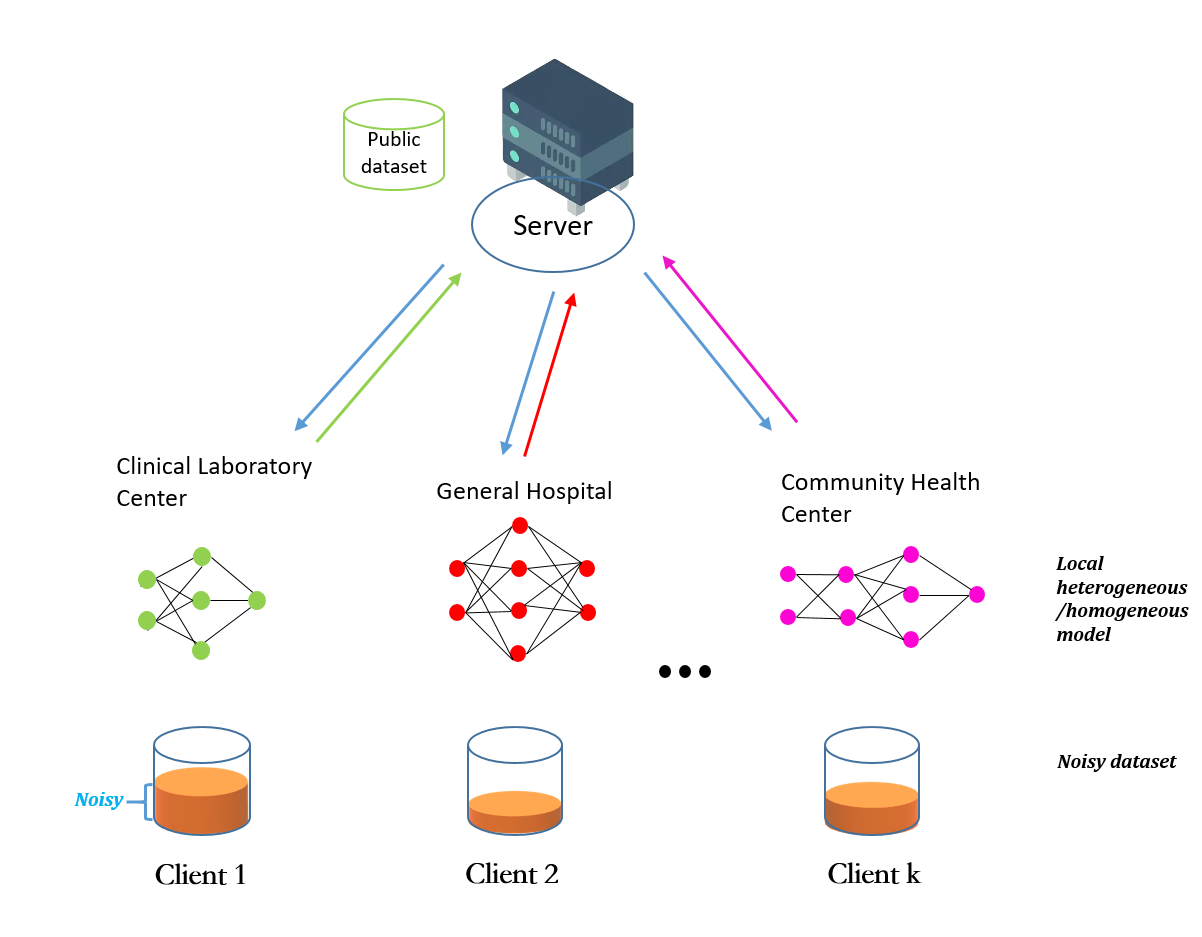
\includegraphics[width=0.8\linewidth,height=0.4\linewidth]{picture/f1.png}}
    \caption{A schematic of federated learning.}
    \label{fig1}
\end{figure}

Federated learning can be classified based on whether the participating datasets are the same, resulting in two types: homogeneous federated
learning  and heterogeneous federated learning \cite{b10},\cite{b11}. In homogeneous federated
learning, all participants have datasets with the same characteristics and data distribution, whereas in heterogeneous federated learning,
participants' datasets may differ in their characteristics and data distribution. The second classification of federated learning is based
on whether the models involved are the same, resulting in two types: horizontal federated learning and vertical
federated learning\cite{b12},\cite{b13}. In horizontal federated learning, all participants have the same model architecture, but may
have different local data\cite{b14}, while in vertical federated learning, each participant has a different model architecture but they collaborate on
processing the same set of data together\cite{b15}. The third way to classify federated learning is based on the type of task involved, resulting in several
types such as federated learning for clustering\cite{b16},\cite{b17}, federated learning for classification\cite{b18},\cite{b19}, federated learning for regression\cite{b20}, among others.
The fourth way to classify federated learning is based on the optimization approach used between the participants, resulting in several types such as
federated averaging\cite{b21},\cite{b22}, federated learning optimization, federated meta-learning\cite{b23}, and so on.

Federated learning methods currently face significant challenges related to their robustness. This article focuses on three main attacks. including backdoor attacks\cite{b24},\cite{b25},\cite{b26},\cite{b27},\cite{b28}, adversarial attacks\cite{b31},\cite{b32},\cite{b33},\cite{b34}, and Byzantine attacks\cite{b29},\cite{b30}. 
A backdoor attack involves a malicious participant in the federated learning process adding a backdoor to the model being trained, which can be triggered by a specific input pattern, 
allowing the attacker to control the output of the model in a targeted way. Adversarial attacks, on the other hand, entail adding small, 
carefully crafted perturbations to the input data to deceive the model and cause it to make incorrect predictions\cite{b31},\cite{b32}.   

\begin{figure}[htbp]
    \centerline{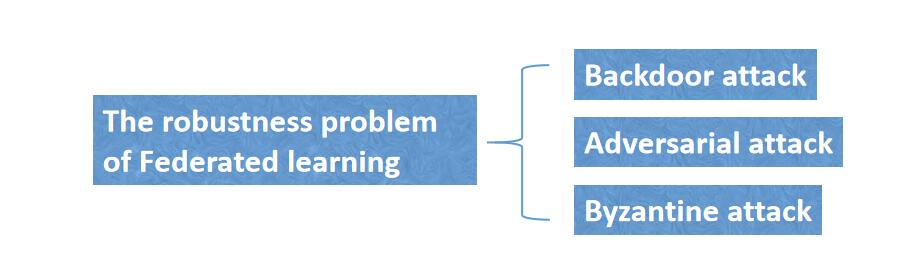
\includegraphics[width=0.8\linewidth,height=0.4\linewidth]{picture/f4.jpg}}
    \caption{The robust threat to federal learning}
    \label{fig2}
\end{figure}
And adversarial attacks can occur in federated learning when a malicious participant intentionally sends adversarial examples to the central server in an attempt to bias the model 
towards their own interests. This can be particularly problematic in applications such as personalized advertising or credit scoring, where the malicious participant may be motivated 
to gain an unfair advantage. Finally, Byzantine attacks involve one or more malicious participants in the federated learning process sending incorrect or misleading updates to the 
central server to disrupt the training process\cite{b35}.  

While federated learning can be vulnerable to certain types of attacks, there are techniques and approaches that can be used to improve the robustness and security of the process. 
It is important to carefully consider these issues when designing and implementing federated learning systems\cite{b38},\cite{b39}. 
For instance, knowledge distillation is a technique that can mitigate backdoor attacks by training a smaller\cite{b36}, 
distilled model using the output of the original model as the target labels. 
This can help remove any backdoor triggers that may have been added to the original model, as the smaller model won't be able to identify them. 
Another technique to mitigate backdoor attacks is model erasure\cite{b44}, where the model is trained to ignore specific input patterns that may be associated with the backdoor.  
\begin{figure}[htbp]
    \centerline{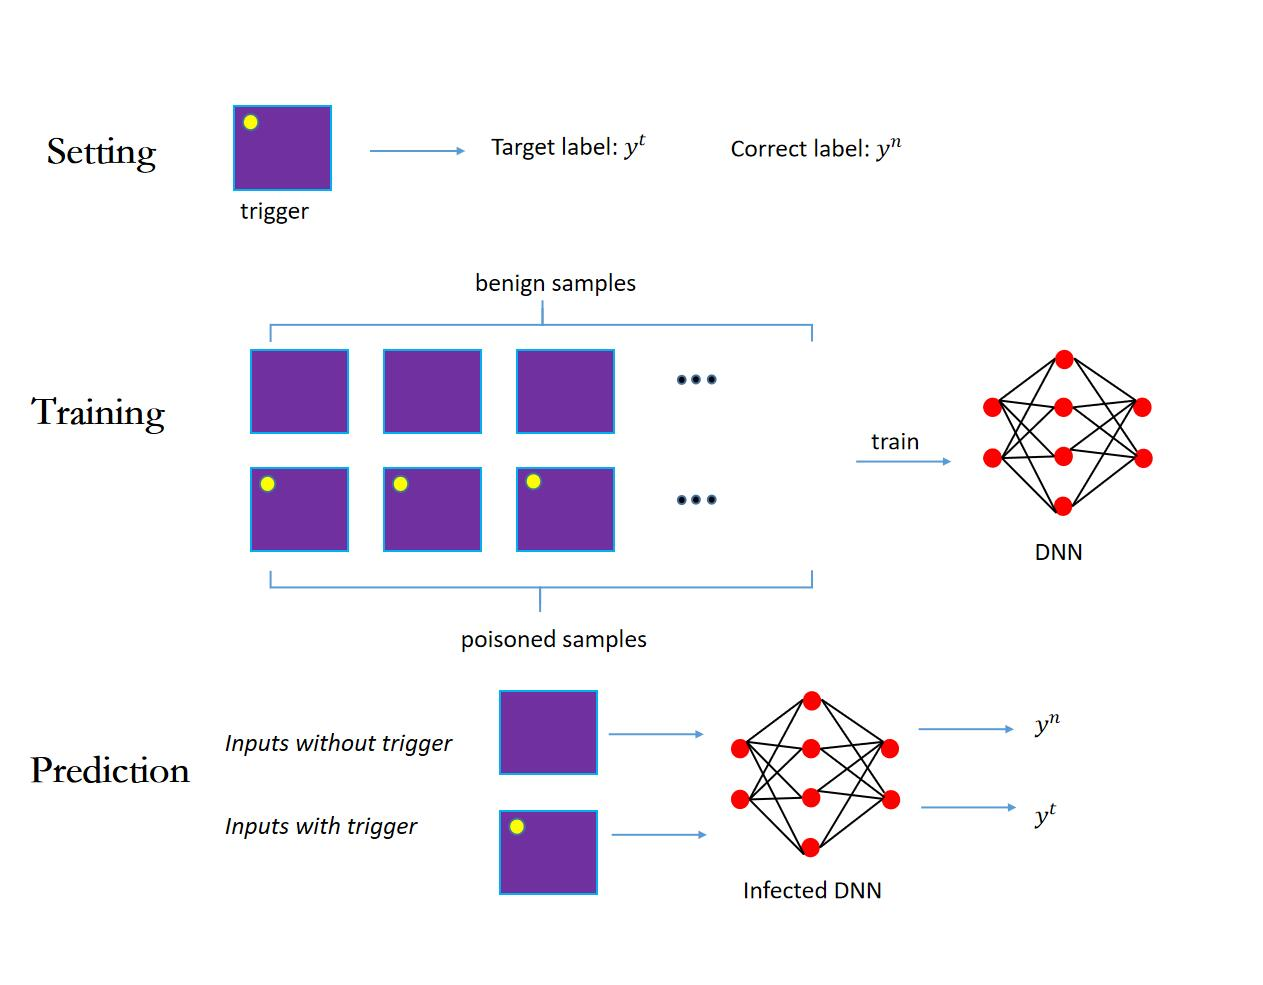
\includegraphics[width=0.8\linewidth,height=0.4\linewidth]{picture/f3.jpg}}
    \caption{Backdoor Attack}
    \label{fig3}
\end{figure}

Adversarial training is a technique that involves explicitly training the model to resist adversarial examples 
by adding adversarial perturbations to the training data\cite{b31},\cite{b32}.  
This can improve the model's ability to detect and resist adversarial attacks in federated learning settings.  
\begin{figure}[htbp]
    \centerline{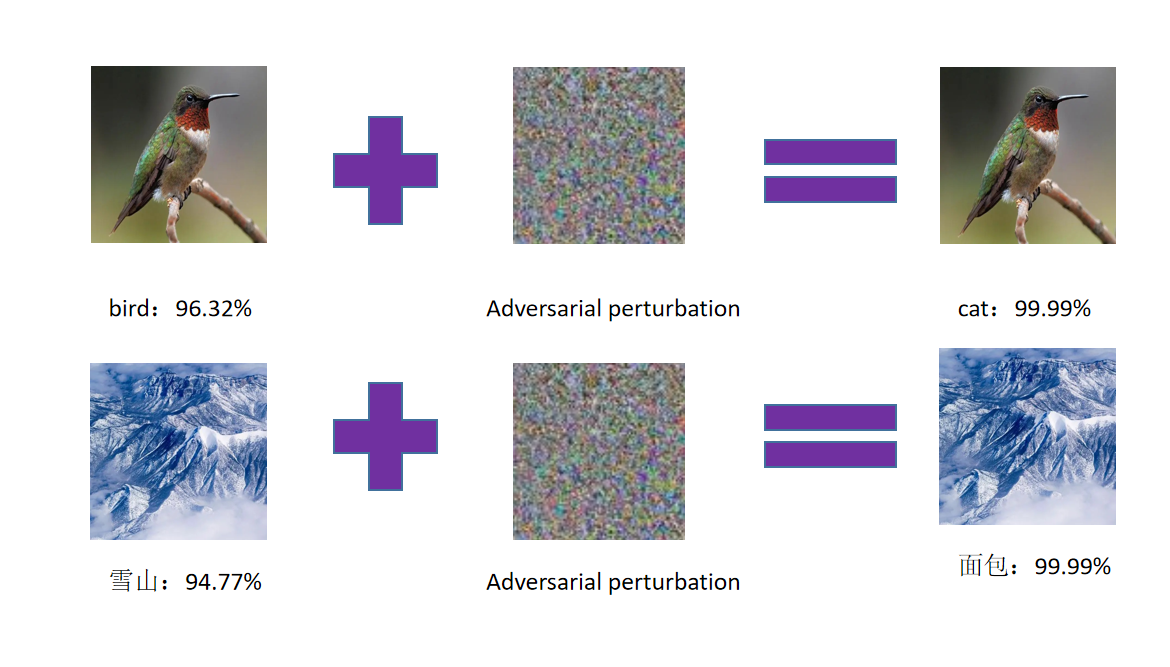
\includegraphics[width=0.8\linewidth,height=0.4\linewidth]{picture/f2.png}}
    \caption{Adversarial Attack}
    \label{fig4}
\end{figure}
Clustering can be used to identify malicious clients in federated learning systems subject to Byzantine attacks\cite{b35},\cite{b36}. 
The idea is to group participating clients based on the similarity of their updates, and to identify any clients whose updates are significantly different from the others. 
These clients can then be excluded from the training process, or their updates can be treated with greater suspicion to minimize the impact of their malicious behavior\cite{b37}.  
\begin{figure}[htbp]
    \centerline{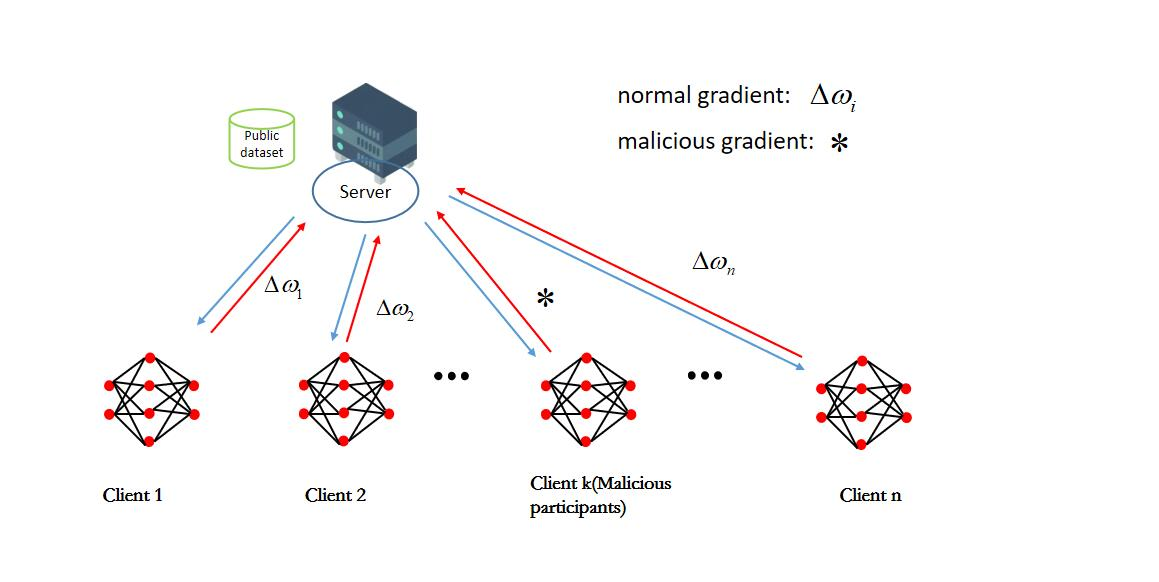
\includegraphics[width=0.8\linewidth,height=0.4\linewidth]{picture/f5.jpg}}
    \caption{Byzantine Attack}
    \label{fig5}
\end{figure}
This paper provides an overview of methods to increase the robustness of federated learning models, with the aim of enhancing the credibility and security of federated learning. 
While previous work has addressed the security of federated learning\cite{b39},\cite{b40},\cite{b41},\cite{b42},\cite{b43}, it has primarily focused on privacy leakage or backdoor attacks, 
with relatively few studies and reports on adversarial attacks. Building on prior work, this paper summarizes the attacks and defense methods of adversarial, backdoor, 
and Byzantine attacks in federated learning. A new classification method is proposed, supplementing the deficiencies of previous work on adversarial attacks. 
Moreover, this paper investigates a multi-level defense system against these attacks, and identifies open problems and future research directions for improving 
the robustness of federated learning.

\section{Thraet Model}
Prior to delving into the details of the threats to federal learning, it is essential
to establish the connections between these threats based on different criteria. 
Specifically, we can categorize these threats into two main stages: 
the training phase and the inference phase. Additionally, we can 
differentiate between untargeted attacks and targeted attacks based 
on whether a specific target is present or not.\cite{b38},\cite{b39},\cite{b40},\cite{b41}.  

\subsection{Training Phase and Inference Phase}  
\subsubsection{Training Phase}Attacks that occur during the model training process are 
intended to either disrupt or impact the federated learning model itself. Backdoors are 
inserted into the model during the training phase to influence the resulting model outcomes\cite{b45},\cite{b46}. 
On the other hand, Byzantine attacks disrupt the convergence of the model by utilizing malicious 
clients or servers\cite{b29}.  
\subsubsection{Inference Phase}Attacks that occur during the reasoning phase are 
typically intended to alter the model's reasoning outcomes and deceive it 
into generating incorrect outputs\cite{b47}. During the training stage, backdoor 
attacks involve the insertion of a backdoor into the model, whereas 
input deception models with triggers are utilized during the 
reasoning stage to cause the model to generate incorrect results. 
Adversarial attacks, on the other hand, leverage the model's vulnerability 
to disturbances and utilize samples with adversarial perturbations as input 
to the model, causing it to produce erroneous outcomes.  

\subsection{Untargeted and Targeted}  
\subsubsection{Untargeted attack}Untargeted attacks are designed to compromise 
the integrity of the target model in an arbitrary manner.
Byzantine attack is one form of an untargeted attack that involves 
uploading malicious gradients to the server in an arbitrary manner, 
with the goal of causing the global model to fail\cite{b48},\cite{b49},\cite{b50},\cite{b51}.
\subsubsection{Targeted Attack}A targeted attack is executed with 
the aim of inducing the model to produce the target label specified by the 
adversary for specific testing examples, while keeping the testing error for 
other testing examples unaffected.




\begin{thebibliography}{00}
    \bibitem{b1} M. Goddard, The EU General Data Protection Regulation (GDPR): European regulation that has a global impact, International Journal of Market Research 59 (2017) 703–705.
    \bibitem{b2} O. Gómez-Carmona, D. Casado-Mansilla, F. A. Kraemer, D. L. de Ipiña, J. GarcíaZubia, Exploring the computational cost of machine learning at the edge for human-centric internet of things, Future Generation Computer Systems 112 (2020) 670–683.
    \bibitem{b3} J. Zhang, D. Tao, Empowering things with intelligence: A survey of the progress, challenges, and opportunities in artificial intelligence of things, IEEE Internet of Things Journal 8 (2021) 7789–7817.
    \bibitem{b4} C. Ma, J. Koneˇcný, M. Jaggi, V. Smith, M. Jordan, P. Richtárik, M. Takáˇc, Distributed optimization with arbitrary local solvers, Optimization Methods and Software 32 (2017) 813–848.
    \bibitem{b5} Brendan McMahan, Eider Moore, Daniel Ramage, Seth Hampson, and Blaise Aguera y Arcas. Communication-Efficient Learning of Deep Networks from Decentralized Data. In Proceedings of the 20th International Conference on Artificial Intelligence and Statistics, volume 54 of Proceedings of Machine Learning Research, pages 1273–1282. PMLR, 20–22 Apr 2017.
    \bibitem{b6} GlobalFederatedLearningMarketbyApplication (Drug Discovery, Industrial IoT, Risk Management), Vertical (Healthcare  Life Sciences, BFSI, Manufacturing, Automotive Transportation, Energy  Utilities), and Region - Forecast to 2028, "researchandmarkets.com", Accessed date: May 12, 2023.
    \bibitem{b7} Q. Yang, Y. Liu, Y. Cheng, Y. Kang, T. Chen, H. Yu, Federated Learning, Synthesis Lectures on Artificial Intelligence and Machine Learning, 2019.
    \bibitem{b8} M. Househ, E. Borycki, and A. Kushniruk. Multiple Perspectives on Artificial Intelligence in Healthcare. Springer, 2021.
    \bibitem{b9} R. Rau, R. Wardrop, and L. Zingales. The Palgrave Handbook of Technological Finance. Springer, 2021.
    \bibitem{b10} Fang, Xiuwen, and Mang Ye. "Robust federated learning with noisy and heterogeneous clients." Proceedings of the IEEE/CVF Conference on Computer Vision and Pattern Recognition. 2022.
    \bibitem{b11} Tang, Zhenheng, et al. "Virtual homogeneity learning: Defending against data heterogeneity in federated learning." International Conference on Machine Learning. PMLR, 2022.
    \bibitem{b12} Kairouz, Peter, et al. "Advances and open problems in federated learning." Foundations and Trends® in Machine Learning 14.1–2 (2021): 1-210.
    \bibitem{b13} Yang, Qiang, et al. "Federated machine learning: Concept and applications." ACM Transactions on Intelligent Systems and Technology (TIST) 10.2 (2019): 1-19.
    \bibitem{b14} Huang, Wei, et al. "Fairness and accuracy in horizontal federated learning." Information Sciences 589 (2022): 170-185.
    \bibitem{b15} Liu, Yang, et al. "Vertical federated learning." arXiv preprint arXiv:2211.12814 (2022).
    \bibitem{b16} Ghosh, Avishek, et al. "An efficient framework for clustered federated learning." Advances in Neural Information Processing Systems 33 (2020): 19586-19597.
    \bibitem{b17} Briggs, Christopher, Zhong Fan, and Peter Andras. "Federated learning with hierarchical clustering of local updates to improve training on non-IID data." 2020 International Joint Conference on Neural Networks (IJCNN). IEEE, 2020.
    \bibitem{b18} Hsu, Tzu-Ming Harry, Hang Qi, and Matthew Brown. "Federated visual classification with real-world data distribution." Computer Vision–ECCV 2020: 16th European Conference, Glasgow, UK, August 23–28, 2020, Proceedings, Part X 16. Springer International Publishing, 2020.
    \bibitem{b19} Wahab, Omar Abdel, et al. "Federated machine learning: Survey, multi-level classification, desirable criteria and future directions in communication and networking systems." IEEE Communications Surveys and Tutorials 23.2 (2021): 1342-1397.
    \bibitem{b20} Yang, Shengwen, et al. "Parallel distributed logistic regression for vertical federated learning without third-party coordinator." arXiv preprint arXiv:1911.09824 (2019).
    \bibitem{b21} Deng, Yuyang, Mohammad Mahdi Kamani, and Mehrdad Mahdavi. "Distributionally robust federated averaging." Advances in neural information processing systems 33 (2020): 15111-15122.
    \bibitem{b22} Sun, Tao, Dongsheng Li, and Bao Wang. "Decentralized federated averaging." IEEE Transactions on Pattern Analysis and Machine Intelligence 45.4 (2022): 4289-4301.
    \bibitem{b23} Fallah, Alireza, Aryan Mokhtari, and Asuman Ozdaglar. "Personalized federated learning: A meta-learning approach." arXiv preprint arXiv:2002.07948 (2020).  
    \bibitem{b24} Bagdasaryan, Eugene, et al. "How to backdoor federated learning." International conference on artificial intelligence and statistics. PMLR, 2020.  
    \bibitem{b25} Wang, Hongyi, et al. "Attack of the tails: Yes, you really can backdoor federated learning." Advances in Neural Information Processing Systems 33 (2020): 16070-16084.   
    \bibitem{b26} Gong, Xueluan, et al. "Backdoor attacks and defenses in federated learning: State-of-the-art, taxonomy, and future directions." IEEE Wireless Communications (2022).  
    \bibitem{b27} Sun, Ziteng, et al. "Can you really backdoor federated learning?." arXiv preprint arXiv:1911.07963 (2019).  
    \bibitem{b28} Ozdayi, Mustafa Safa, Murat Kantarcioglu, and Yulia R. Gel. "Defending against backdoors in federated learning with robust learning rate." Proceedings of the AAAI Conference on Artificial Intelligence. Vol. 35. No. 10. 2021.  
    \bibitem{b29} Fang, Minghong, et al. "Local model poisoning attacks to {Byzantine-Robust} federated learning." 29th USENIX security symposium (USENIX Security 20). 2020.  
    \bibitem{b30} Guo, Shangwei, et al. Byzantine-Resilient Decentralized Stochastic Gradient Descent.  
    \bibitem{b31} Zizzo, Giulio, et al. "Fat: Federated adversarial training." arXiv preprint arXiv:2012.01791 (2020).  
    \bibitem{b32} Chen, Chen, et al. "Calfat: Calibrated federated adversarial training with label skewness." Advances in Neural Information Processing Systems 35 (2022): 3569-3581.  
    \bibitem{b33} Li, Xiaoxiao, Zhao Song, and Jiaming Yang. "Federated adversarial learning: A framework with convergence analysis." International Conference on Machine Learning. PMLR, 2023.  
    \bibitem{b34} Zhang, Jie, et al. "Delving into the adversarial robustness of federated learning." arXiv preprint arXiv:2302.09479 (2023).  
    \bibitem{b35} Prakash, Saurav, and Amir Salman Avestimehr. "Mitigating byzantine attacks in federated learning." arXiv preprint arXiv:2010.07541 (2020).   
    \bibitem{b36} Huang, Hanxun, et al. "Distilling Cognitive Backdoor Patterns within an Image." arXiv preprint arXiv:2301.10908 (2023).   
    \bibitem{b37} Blanchard, Peva, et al. "Machine learning with adversaries: Byzantine tolerant gradient descent." Advances in neural information processing systems 30 (2017).   
    \bibitem{b38} Lyu, Lingjuan, et al. "Privacy and robustness in federated learning: Attacks and defenses." IEEE transactions on neural networks and learning systems (2022).    
    \bibitem{b39} Guo, Shangwei, et al. "Robust and privacy-preserving collaborative learning: A comprehensive survey." arXiv preprint arXiv:2112.10183 (2021).    
    \bibitem{b40} Enthoven, David, and Zaid Al-Ars. "An overview of federated deep learning privacy attacks and defensive strategies." Federated Learning Systems: Towards Next-Generation AI (2021): 173-196.  
    \bibitem{b41} Rodríguez-Barroso, Nuria, et al. "Survey on federated learning threats: Concepts, taxonomy on attacks and defences, experimental study and challenges." Information Fusion 90 (2023): 148-173.  
    \bibitem{b42} Tariq, Asadullah, et al. "Trustworthy Federated Learning: A Survey." arXiv preprint arXiv:2305.11537 (2023).   
    \bibitem{b43} Zhang, Yifei, et al. "A Survey of Trustworthy Federated Learning with Perspectives on Security, Robustness, and Privacy." arXiv preprint arXiv:2302.10637 (2023).  
    \bibitem{b44} Dal Fabbro, Nicolò, Aritra Mitra, and George J. Pappas. "Federated TD Learning over Finite-Rate Erasure Channels: Linear Speedup under Markovian Sampling." IEEE Control Systems Letters (2023).  
    \bibitem{b45} Miao, Chenglin, et al. "Towards data poisoning attacks in crowd sensing systems." Proceedings of the Eighteenth ACM International Symposium on Mobile Ad Hoc Networking and Computing. 2018.  
    \bibitem{b46} Zhang, Hengtong, et al. "Data poisoning attack against knowledge graph embedding." arXiv preprint arXiv:1904.12052 (2019).   
    \bibitem{b47} Barreno, Marco, et al. "Can machine learning be secure?." Proceedings of the 2006 ACM Symposium on Information, computer and communications security. 2006.  
    \bibitem{b48} Lamport, Leslie, Robert Shostak, and Marshall Pease. "The Byzantine generals problem." Concurrency: the works of leslie lamport. 2019. 203-226.   
    \bibitem{b49} Xie, Cong, Oluwasanmi Koyejo, and Indranil Gupta. "Fall of empires: Breaking byzantine-tolerant sgd by inner product manipulation." Uncertainty in Artificial Intelligence. PMLR, 2020.  
    \bibitem{b50} Bernstein, Jeremy, et al. "signSGD with majority vote is communication efficient and fault tolerant." arXiv preprint arXiv:1810.05291 (2018).  
    \bibitem{b51} Damaskinos, Georgios, et al. "Aggregathor: Byzantine machine learning via robust gradient aggregation." Proceedings of Machine Learning and Systems 1 (2019): 81-106.










\end{thebibliography}


\end{document}